\chapter{Sample Analysis and Conclusion}
\label{sec:chapter_2}

After explanation of the system architecture and hardware design, the test methodology and the analysis of the results from the hardware is defined. The results are captured thanks to ChipScope software which help for internal acquisitions in various points of the Programmable Logic of FPGA. There are other tests we did to have an estimation of the system in total. For instance, we send a random data stream from a PC and send it via Ethernet in different packet size to a board and compare it in another PC where we generate the same random set.\\

\section{Hardware Samples and Analysis}
\label{hw_samples}

A complete OFDM frame is illustrated in Figure \ref{ofdmframe_chipscope}. The position of preamble signal is completely distinguished in the figure which is comparable of the standard shown in previously except the \textit{Training}. This section is special for our design for conveying some further information about the node. The detail of each preamble word is zoom in the next figures as defined in Section \ref{section:ieee_standard}. Specifically, the STS section is shown in Figure \ref{sts_chipscope}.\\
\begin{figure}
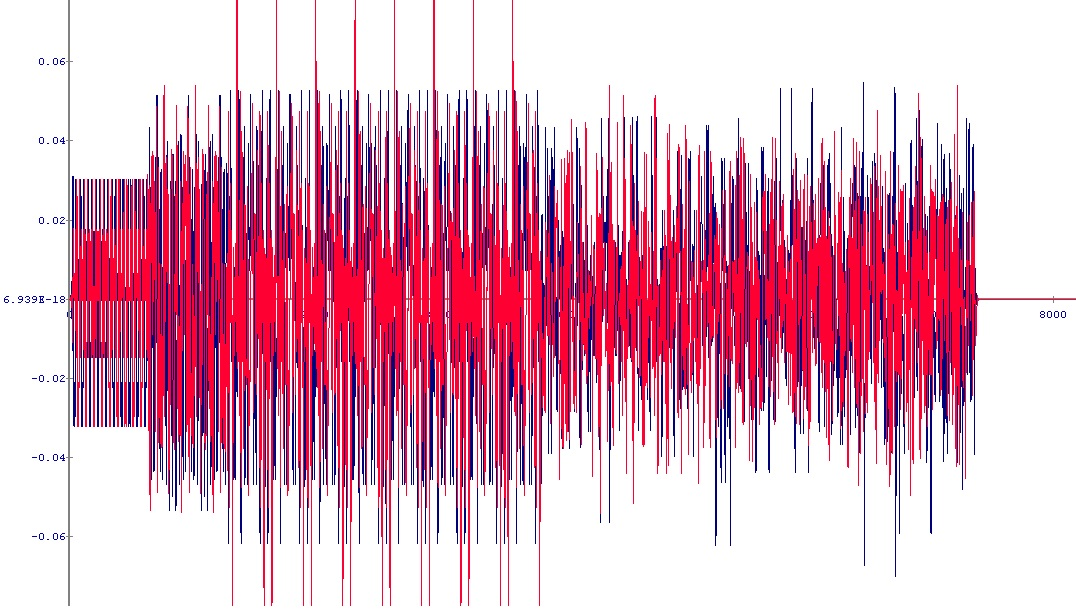
\includegraphics[width=\textwidth]{content/fig/ofdmframe_chipscope.JPG}
\caption{OFDM Frame (I/Q) detected in Chipscope.}
\label{fig:ofdmframe_chipscope}
\end{figure}

\begin{figure}
\centering
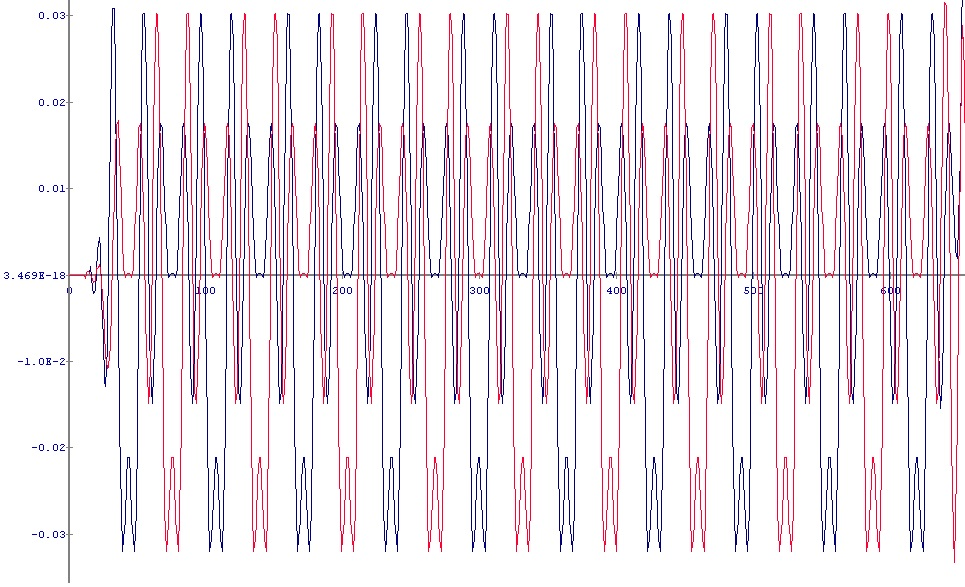
\includegraphics[width=12cm]{content/fig/sts_chipscope.JPG}
\caption{STS (I/Q) detected in Chipscope.}
\label{fig:sts_chipscope}
\end{figure}

The auto-correlation is perform to catch the begining of the preamble with is STS. The output of the block is shown in Figure \ref{autocorr} to detect the signal arrival.\\

\begin{figure}
\centering
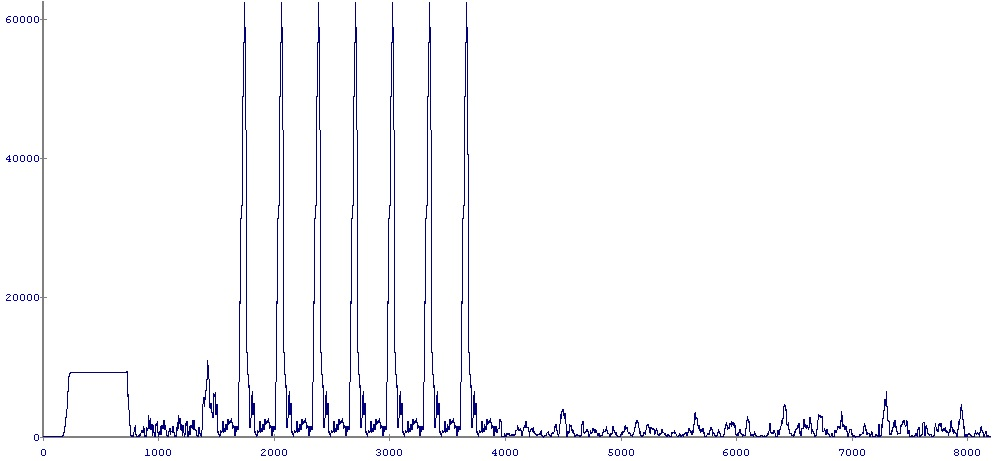
\includegraphics[width=\textwidth]{content/fig/autocorr.JPG}
\caption{Auto-Correlation detected in Chipscope.}
\label{fig:autocorr}
\end{figure}

The cross-correlation on the LTS with a pre-defined expected LTS is shown in Figure \ref{crosscorr}. As already described we have 2.5 LTS symbol in each frame. So, two peak are detected in the system.\\

\begin{figure}
\centering
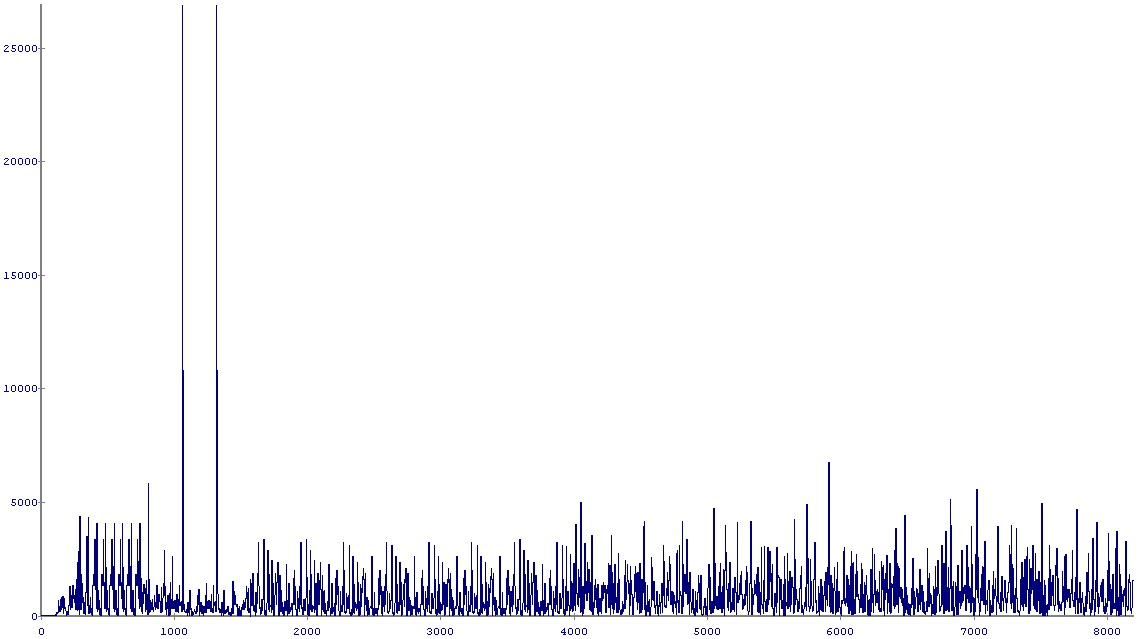
\includegraphics[width=\textwidth]{content/fig/crosscorr.JPG}
\caption{Cross-Correlation detected in Chipscope.}
\label{fig:crosscorr}
\end{figure}

The LTS section is supposed to carry a flat shape in frequency that is used for the channel response estimation. In the Figure \ref{baseIFAdcDac} shows the frequency response of the LTS in the in the input of the receiver side. Beginning of the system test, we make a loop after the DAC of the transmitter to the ADC of the receiver and the is no RF conversion. Practically, this shape represents the frequency response of the ADC/ DAC and some non-linear elements like induction and trances. Because, there are some trances in the path who rejects the DC frequencies we needed to use an IF filter to modulate the signal around $5 MHz$.\\

\begin{figure}
\centering
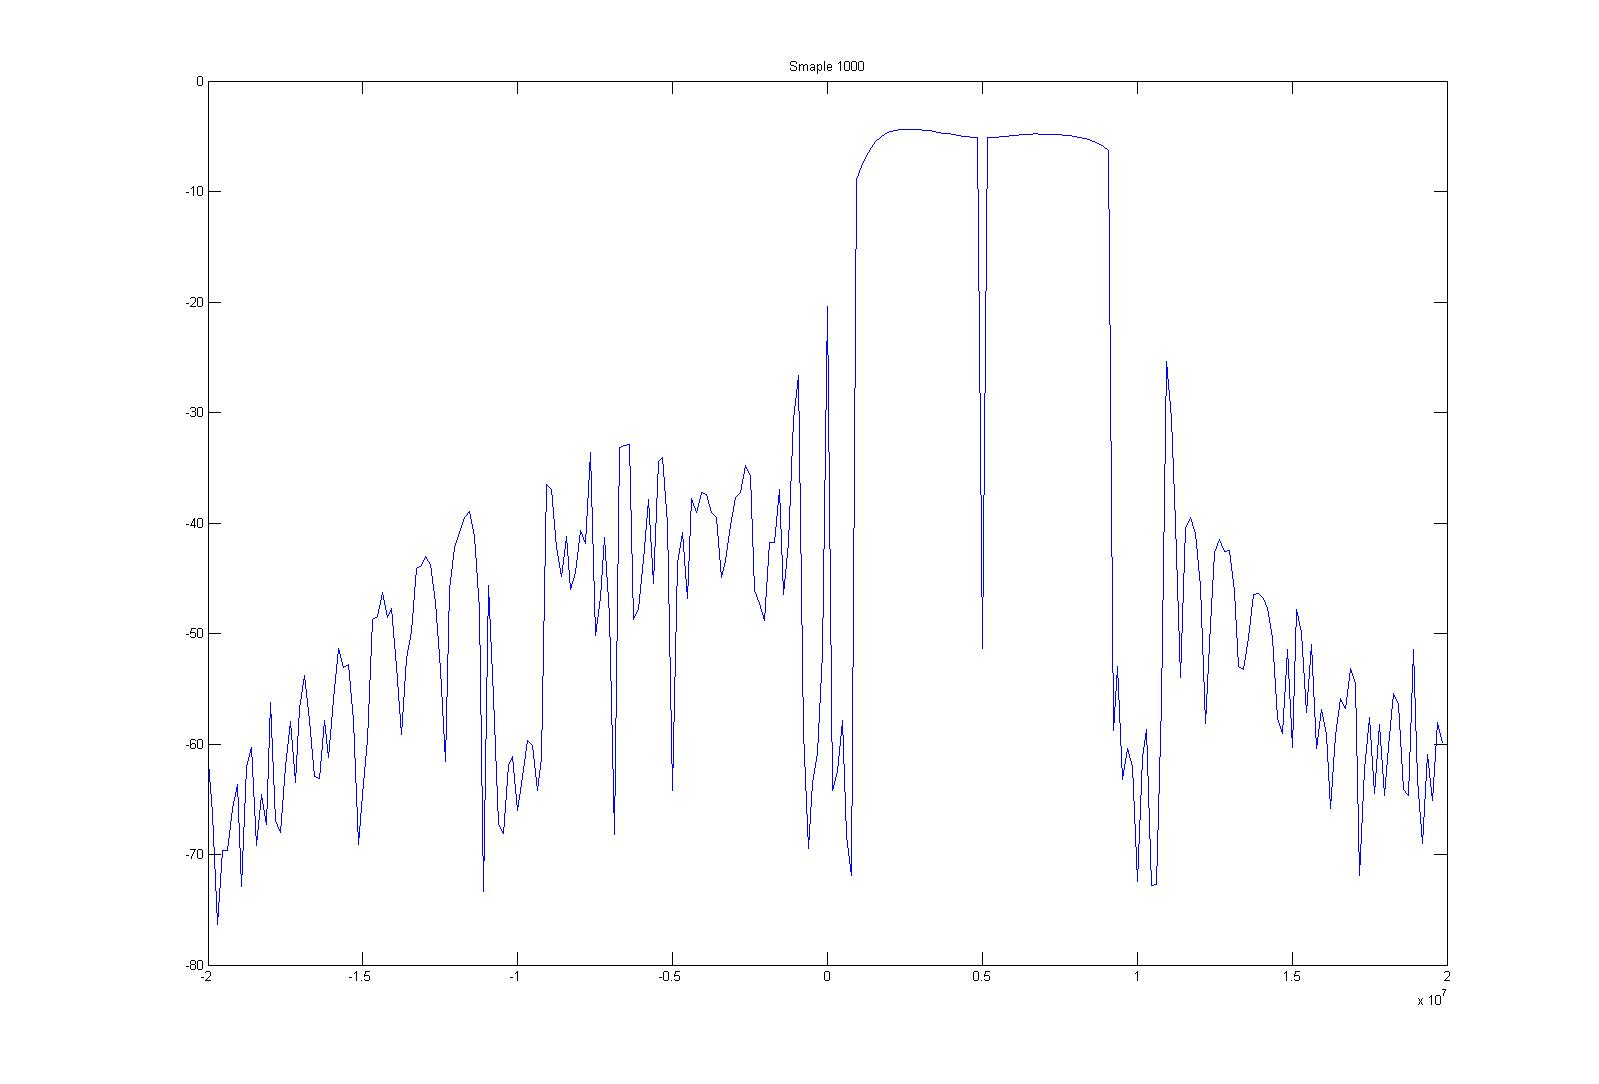
\includegraphics[width=10cm]{content/fig/baseIFAdcDac.JPG}
\caption{LTS Spectrum in Baseband chain (IF filter on 5MHz is enable)}
\label{fig:baseIFAdcDac}
\end{figure}

Passing the signal through the RF side which modulate around $2.4 GHz$ and demodulate it again we have a shape as shown in Figure \ref{RfIF}. As you can see we still have the IF filter. The peak on 0 frequency is a result of the electronic elements which injects DC.\\

\begin{figure}
\centering
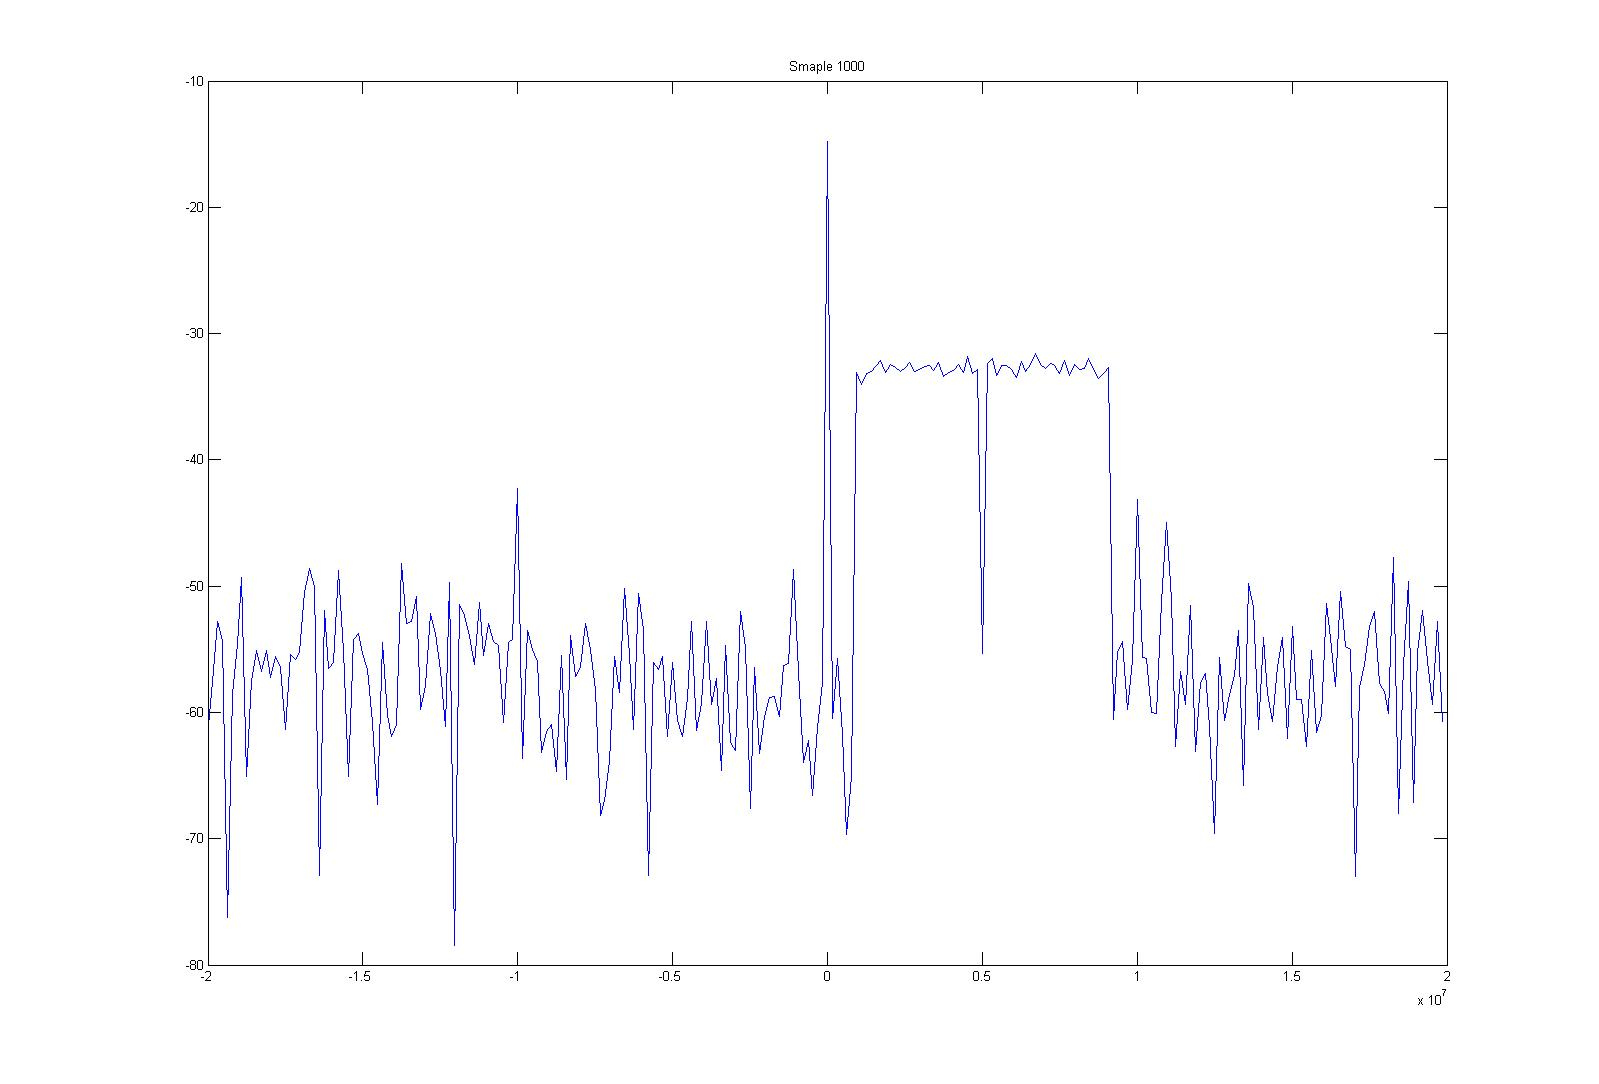
\includegraphics[width=10cm]{content/fig/RfIF.JPG}
\caption{LTS Spectrum- passed RF chain (IF filter  on 5MHz is enable)}
\label{fig:RfIF}
\end{figure}

We have a shape of LTS frequency response like Figure \ref{Rfbase} if the IF filter is not activated. As you can see we have the DC peak which can be rejected easily.\\

\begin{figure}
\centering
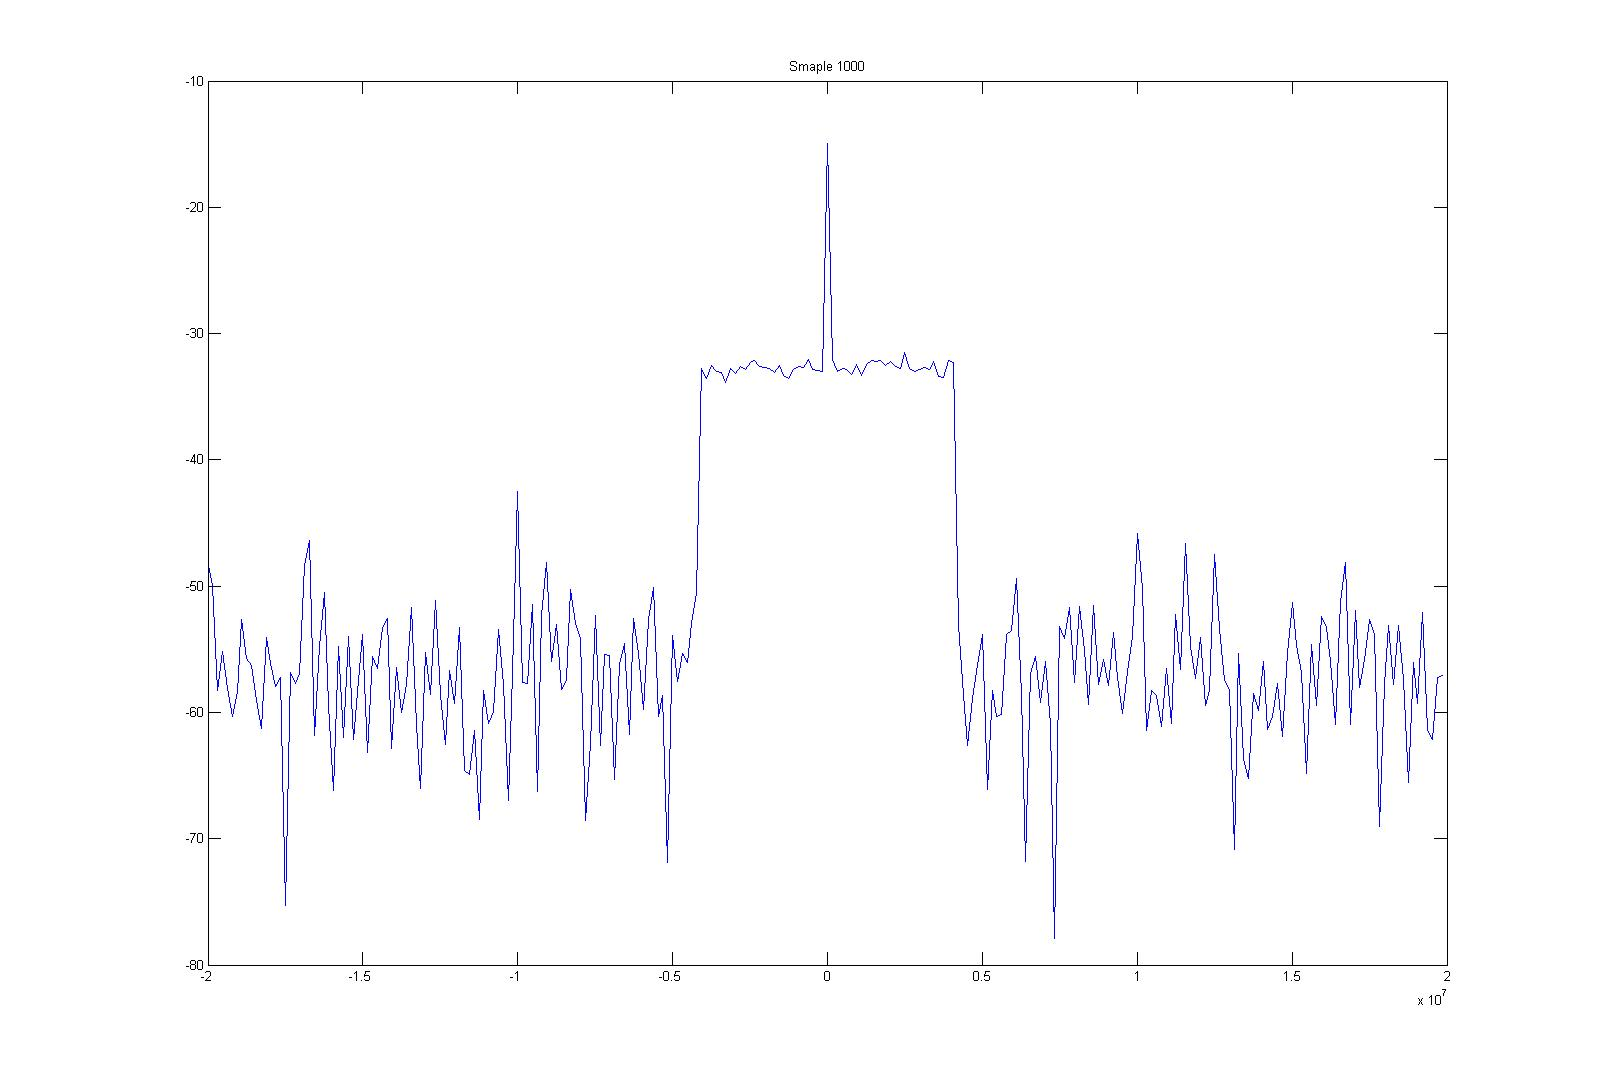
\includegraphics[width=10cm]{content/fig/Rfbase.JPG}
\caption{LTS Spectrum- passed RF chain (IF filter is disable)}
\label{fig:Rfbase}
\end{figure}

Figure \ref{h_mag_chipscope_noChannel} is the frequency response of the channel after an internal loop between the transmitter and the receiver on one FPGA board. As it is a perfect channel without any distortion we just have a perfect flat estimation of the channel. This response is used to compensate all the signal tones.\\

\begin{figure}
\centering
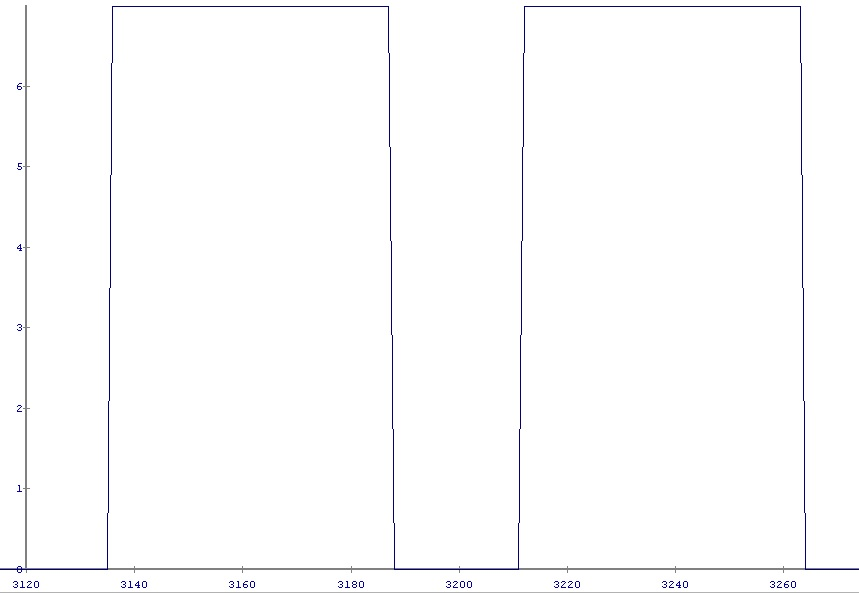
\includegraphics[width=10cm]{content/fig/h_mag_chipscope_noChannel.JPG}
\caption{Frequency Response of a perfect channel detected in Chipscope}
\label{fig:h_mag_chipscope_noChannel}
\end{figure}

Figure \ref{h_mag_chipscope_rf_detect} in a real channel after all the conversions of the transmitter and the receiver. The RF chain is activated in the scenario. Interestingly, we have a perfect detection of the symbols even after such the distortion.\\

\begin{figure}
\centering
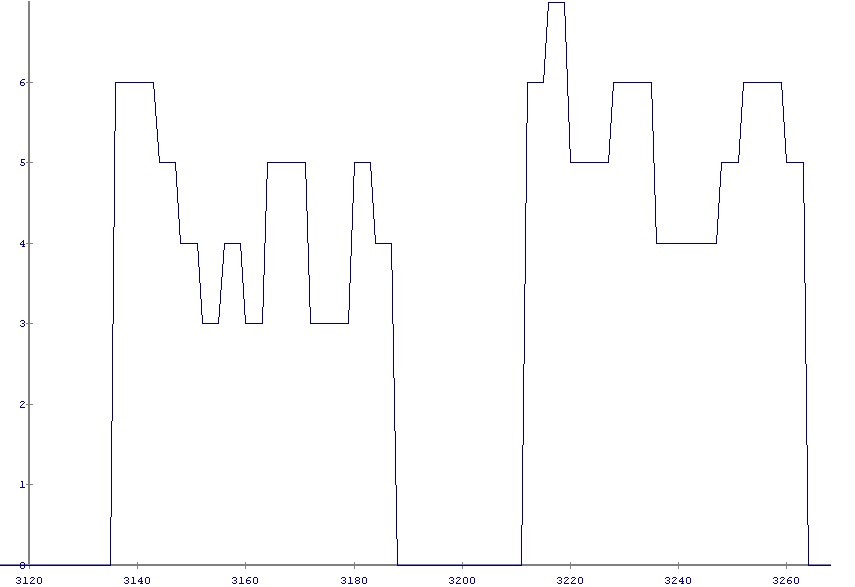
\includegraphics[width=10cm]{content/fig/h_mag_chipscope_rf_detect.JPG}
\caption{Frequency Response of on air channel detected in Chipscope}
\label{fig:h_mag_chipscope_rf_detect}
\end{figure}

\begin{figure}
\centering
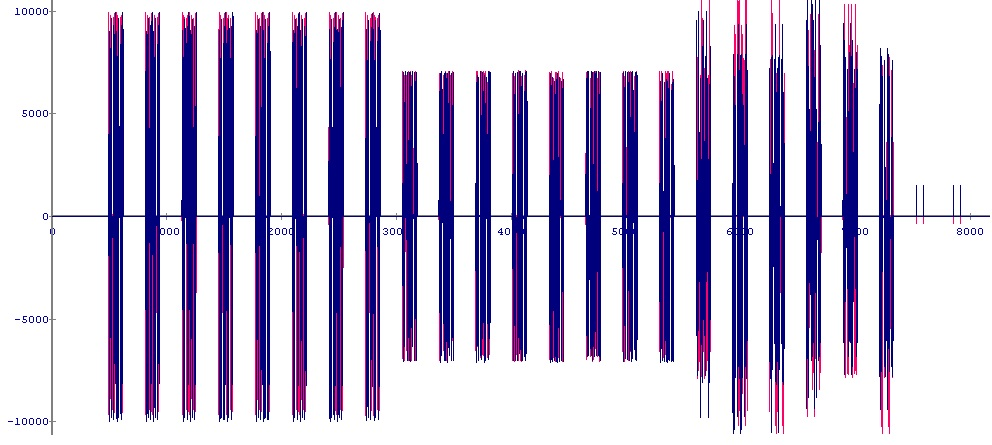
\includegraphics[width=\textwidth]{content/fig/OfdmSym_16qam_1_2_code_64byte.JPG}
\caption{OFDM Symbols of a 16QAM 64-byte message Coded 1/2 rate}
\label{fig:OfdmSym_16qam_1_2_code_64byte}
\end{figure}

Figures \ref{OfdmSym_16qam_1_2_code_64byte} and \ref{OfdmSym_16qam_no_code_64byte} compares two OFDM frames after the FFT block on the receiver side. The coding algorithm is a convolutional code which borrowed from another model and seen as a black-box for our system. Just do not consider the first 8 symbols because they are the training block which are not defined in the standard and are the customization on our specific application. The next 8 frames in the coded and 4 in the non-coded are the base rate frames to report to the receiver about the modulation, size of message, sequence number and some other detection information. the rest are the message and the valuable information for the higher levels of the system.\\

\begin{figure}
\centering
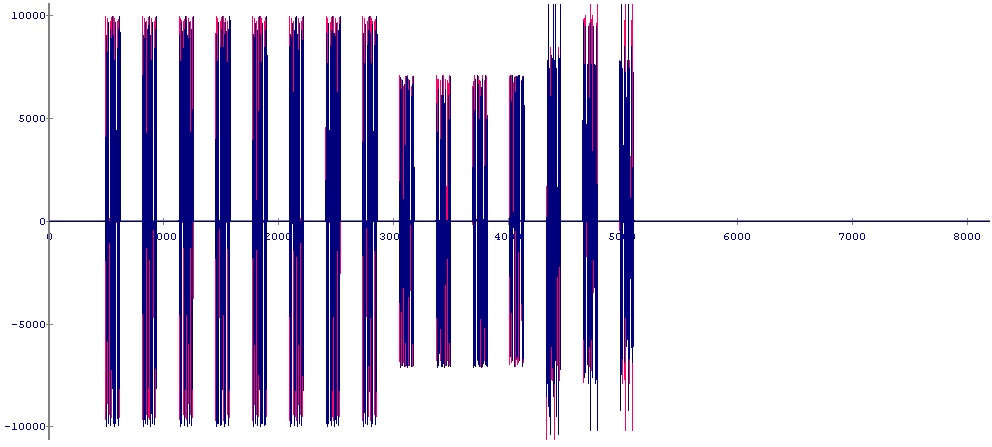
\includegraphics[width=\textwidth]{content/fig/OfdmSym_16qam_no_code_64byte.JPG}
\caption{OFDM Symbols of a 16QAM 64-byte message no-Coded}
\label{fig:OfdmSym_16qam_no_code_64byte}
\end{figure}

\section{Bit-Error Rate Calculation}
Will be add later!!!


\section{FPGA Resource Consumption}
The device used in our implementation is  XC7Z045-22FFG900C and in Table \ref{table:DevUtil} you can find the device utilization:\\


\begin{table}
\centering
\vspace{0.5cm}
\begin{tabular}{c|c|c|c}
Slice Logic Utilization&Used&Available&Utilization\\ \hline
Number of Slice Registers&42,703&437,200&9\% \\
Number of Slice LUTs&59,787&218,600&27\% \\
Number used as Memory&5,384&70,400&7\% \\
Number of occupied Slices&21,749&54,650&39\% \\
Number of DSP48E1s&149&900&16\% \\
\end{tabular}

\caption{Device Utilization Summary (actual values)}
\label{table:DevUtil}
\end{table}

Keep in mind this table shows all the utilization of the ADC/DAC interface, BRAM, clock generator and OFDM PHY module. For OFDM PHY module we could reach Net Skew 0.51 ns and maximum  Delay $1.91 ns$. About the ARM processor, we used one of the ARM cores although we have a dual core architecture. It works with $666.6 MHz$ clock. It is almost 20\% of the processor.\\

\section{Conclusion}

This thesis has presented the theoretical analysis and simulation and  FPGA implementation details of a baseband OFDM system with channel estimation and timing synchronization. A radio board also is explained for the practical usage and proof of the feasibility. The OFDM system is prototyped based on IEEE 802.11a standard and transmits/receives signals on a 20 MHz bandwidth. The conceptual design is done in System Generator and ported on a FPGA. With QPSK modulation scheme, the system achieves a throughput of 24 Mbps.\\
Another critical part of the project is to reach an acceptable communication bit-rate in the processor side to the peripherals, more specifically Ethernet, for conveying data between two PC which is done perfectly.\\

\subsection{Future Work}
No doubt, System Generator is a very powerful tool for conceptual proof but is not still an industrial support. There are still difference in the Simulation in Matlab and what we have in the hardware. To overcome this issue we needed to make some changes to have a logical margin of the hardware difficulties. The resource consumption is not very optimized which expected to have better performance using VHDL programming. There are many low-level techniques to manage the power, speed and area which is not applicable in the system.\\
Some other problems like model-based system maintenance, extend for the future and the bug detection difficulties make us to hesitate to industrialized a System Generator model at the moment. However, the accuracy of the theory is done perfectly in the current mechanism.\\
There are some projects in the department to extend the model for MIMO system design which is a good starting point. Besides, they try to upgrade the FFT point to higher levels for better bandwidth usage. A customized radio board is in the future program activities.\\